% \colorlet{chaptergrey}{gray}
% \chapter[Kinematically misaligned galaxies in MaNGA]{Kinematic misalignment in MaNGA}
% \label{ch:halo_assembly}
% \vspace{-5.25in}
% 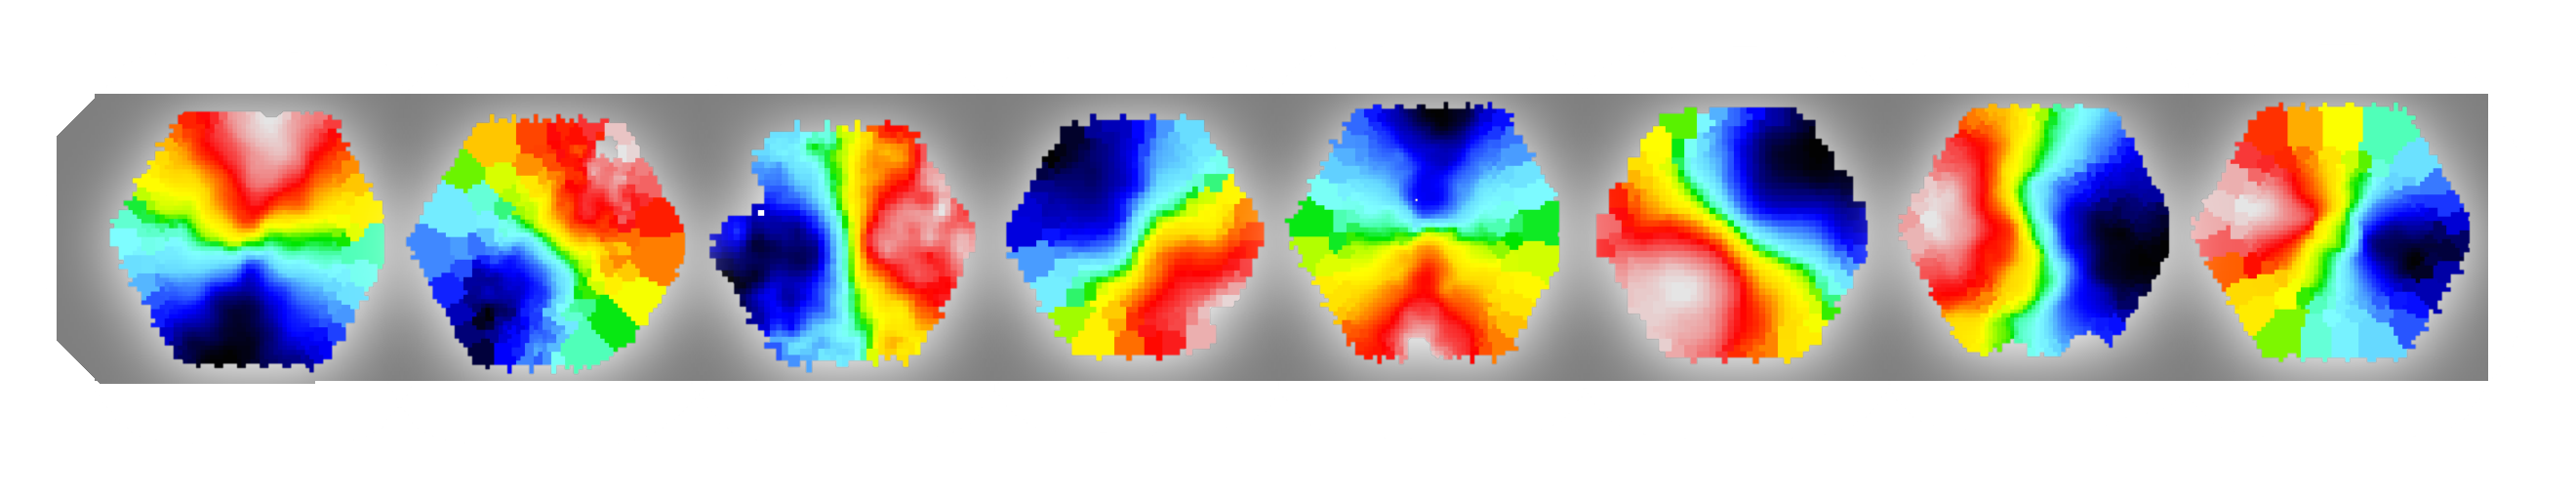
\includegraphics[height=1.39in]{thesis/latex/misalignment_intro/kin_mis_chapter_heading_grey.pdf}
% \vspace{3in}

% \epigraph{This chapter is based on Duckworth, Tojeiro and Kraljic, in MNRAS, 492, Issue 2, 2020. Here we investigate the relationship of kinematically misaligned galaxies with morphology, angular momentum and gas content in observations.}

% \section{Introduction}

% \red{balance introduction section with actual introduction. maybe shorthand here relating gas properties and angular momentum to kinematic misalignment.}

% In this chapter the relationship of kinematic misalignment with optical morphology, angular momentum and gas content is presented in observations. \S\ref{sec:data_obs} gives a description of the additional data catalogues used in this work and \S\ref{sec:results_obs} describes the observational properties of misaligned galaxies.

% \red{talk about MPL-8}

% \section{Data} \label{sec:data_obs}
% This section describes the catalogues crossed matched with the MaNGA sample to seperate galaxies based on optical morphology and group membership.

% \subsection{Morphology} \label{sec:morph_def_obs}
% We classify the morphology of MaNGA galaxies through the formalism laid out by the citizen science project; GalaxyZoo2 \citep[GZ2;][]{willett2013}. GZ2 provides visually identified morphologies (and also measures finer morphological features e.g. bars, bulge size and edge-on discs) for 304,122 galaxies drawn from SDSS. GZ2, however, is not complete for the MaNGA sample and has been combined with an unpublished version; GalaxyZoo4 to provide a consistent set of definitions for all MaNGA targets (see \url{https://www.sdss.org/dr15/data_access/value-added-catalogs/?vac_id=manga-morphologies-from-galaxy-zoo}). 

% In a nutshell, GZ2 provides morphological classification through a decision tree of questions. Further questions are dependent on the answer to the previous to characterise a certain morphological type and identify finer features (see Figure 1 in \citet{willett2013} for this flowchart). From this, a table of vote fractions for each question combined with the total number of votes dictate a reliably sampled galaxy population with a set of desired morphological features. Votes by individuals are debiased (weighted) based on their reliability in comparison to known answers to the questions.

% The first question in the decision tree 'Is the galaxy smooth and rounded with no sign of a disc?', allows categorisation into broad ETGs and LTGs. We select galaxies with a debiased vote fraction > 0.7 for smooth to be ETGs and galaxies with a debiased vote fraction of > 0.7 for disc or features to be LTGs. Defining an exact population of lenticular galaxies (S0s) is tricky through public classifications. LTGs, however, can be separated based on the dominance of the bulge with respect to the disc in GZ2 through the question 'How prominent is the central bulge, compared with the rest of the galaxy?'. \citet{willett2013} demonstrate a strong correlation between bulge dominance as defined per this question and expert classifications of T-type \citep{nair2010}. Equation 19 of \citet{willett2013} provides a linear mapping from GZ2 bulge classification to expert defined morphological T-type. Care must be taken in using this linear mapping \citep[see discussion in][]{willett2013}, however, this should be a reasonable parameterisation to coarsly separate LTGs into earlier-type (S0 - Sa) and later-type spirals (Sb - Sd). We split our LTG population at T-type = 3, to give two morphological categories; S0-Sas and Sb-Sds in addition to pure ETGs.
% % We split our LTG population at T-type = 3, to give three morphological categories along with pure ETGs. 

% The estimates of gas mass used here for MaNGA are derived from the Pipe3D pipeline \citep{pipe3Da, pipe3Dvac}, which uses dust attenuation within the footprint of the IFU, which methodology is described in \citet{barrera2018}.

% \subsection{Group membership} \label{sec:group_def}
% \red{either put full description here or in halo assembly section.}
% To investigate different pathways leading to kinematic misalignment, we must separate galaxies into centrals and satellites. We identify groups with an adaptive halo-based group finder of \citet{yang2005,yang2007} and with improved halo mass assigning techniques \citep[see;][for details and application to SDSS]{lim2017}. In a nutshell, the group finder uses either the stellar mass or luminosity of central galaxies in addition with the $\mathrm{n^{th}}$ brightest/most massive satellite as proxies for halo mass. Galaxies are assigned to groups through an iterative process, where halo properties such as halo size and velocity dispersion are updated until membership converges. 

% % For groups that are outside of the redshift limit where groups are complete final halo masses are assigned through abundance matching. Those incomplete are assigned halo masses based on the ranking between halo mass and the proxy found at the final iteration of the group finder.
% % The performance of the group finder has been tested on realistic mock catalogues, showing that the halo masses of individual haloes are consistent with the true mass with a typical scatter of $\sim$0.2 dex. This scatter is similar to the commonly used group finder of \citet{yang2007}, however extends uniformly to halo masses 0.7 dex lower. 

% % For this work, we use the stellar mass based halo mass proxy for the SDSS main sample. 
% \citet{lim2017} do not apply the group finder to the thin strips in the Southern Galatic Cap of SDSS main due to incomplete groups resulting from close proximity to borders. MaNGA galaxies in these strips are therefore unclassified by the group finder, resulting in 5088 matched galaxies with group membership classifications into central or satellite. 


% \section{Results} \label{sec:results_obs}
% \red{redefine NGRs}
% We divide our MaNGA $\Delta$PA defined population at $\Delta$PA = 30$^{\circ}$ into aligned and misaligned. In the following, we also consider galaxies with defined stellar PAs but undefined H$\alpha$ due to central depletion or incoherent rotation/dispersion domination (no gas rotation; NGRs). Figure \ref{fig:delPA_stelM} shows the distribution of stellar mass for these three populations. We see no significant difference between the aligned and misaligned galaxies, however NGRs appear to be slightly more massive. \citet{graham2018} previously demonstrated the tight correlation between stellar angular momentum and stellar mass for MaNGA ($\sim$2300 galaxies). Since NGRs and misaligned galaxies are slightly higher mass, it could be expected that they are typically less rotationally supported with respect to the $\Delta$PA defined populations. 

% \begin{figure}
%     \centering
% 	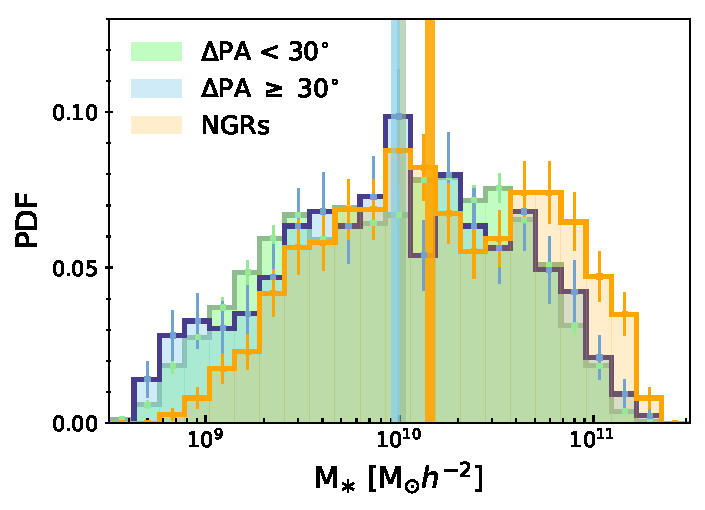
\includegraphics[width=0.7\linewidth]{thesis/latex/misalignment_MaNGA/delPA_stelM.pdf}
%     \caption{Probability density distributions of stellar mass, $\mathrm{(M_{\ast}/M_{\odot})}$ for aligned galaxies ($\Delta$PA < 30$^{\circ}$) shown in green, those with high misalignment ($\Delta$PA > 30$^{\circ}$) are in blue and NGRs are in orange. Each histogram is given with Poisson errors on each bin. The vertical lines denote the corresponding distribution's median. NGRs are typically at higher stellar mass than those with aligned star and gas rotation.}
%     \label{fig:delPA_stelM}
% \end{figure}

% Here we use the luminosity weighted stellar angular momentum estimator, $\mathrm{\lambda_R}$, taken directly from Equation 1 in \citet{emsellem2007} as
% \begin{equation}
% \mathrm{\lambda_{R} \equiv \frac{\langle R | V | \rangle}{ \langle R \sqrt{ V^{2} + \sigma^{2} } \rangle } = \frac{ \Sigma_{ n = 1 }^{ N } F_{ n } R_ { n } \left| V_{ n } \right| }{ \sum_{ n = 1 }^{ N } F_{n} R_{ n } \sqrt{ V_{ n }^{ 2 } + \sigma_{ n }^{ 2 } } }.}
% \end{equation}
% $\mathrm{\lambda_R}$ is calculated from summing over N pixels in the IFU observation within the radius of interest, $\mathrm{R}$. $\mathrm{F_{n}}$, $\mathrm{V_{n}}$ and $\mathrm{\sigma_{n}}$ are the flux, line of sight velocity and line of sight velocity dispersion of the $\mathrm{n^{th}}$ pixel. Here we present all measures of $\mathrm{\lambda_R}$ encompassing a radius of $\mathrm{1.5R_e}$ weighted by $r-$band flux. We also take the ellipticity to be $\mathrm{\epsilon = 1 - b/a}$ where $a$ and $b$ are the major and minor axes of the galaxy estimated from the NASA Sloan Atlas catalogue \cite[used for target selection in MaNGA;][]{blanton2011}.

% Figure \ref{fig:delPA_lambda_Re}, shows $\mathrm{\lambda_R}$ vs $\mathrm{\epsilon}$ for all $\Delta$PA defined galaxies and the medians for the aligned, misaligned and NGR samples. The black solid line overlaid shows the slow rotator regime (enclosed in bottom left). The fast/slow rotator classification refers to whether a given galaxy's rotation can be considered regular (circular velocity) or exhibits dispersion dominated motion \citep[][]{emsellem2007}. Kinematically aligned galaxies reside at preferentially higher $\mathrm{\lambda_R}$ and ellipticity with respect to NGRs. This is indicative of the dispersion dominance over rotation for disrupted gas poor and typically higher mass galaxies that we see in our NGR sample. Interestingly, kinematically misaligned galaxies also typically reside close to the slow rotator regime. In addition, the same qualitative trends are seen (i.e. misaligned and NGR galaxies have lowered angular momentum with respect to the aligned) are seen if this plot is made for ETGs, S0-Sas or Sb-Sds alone. 

% \begin{figure}
%     \centering
% 	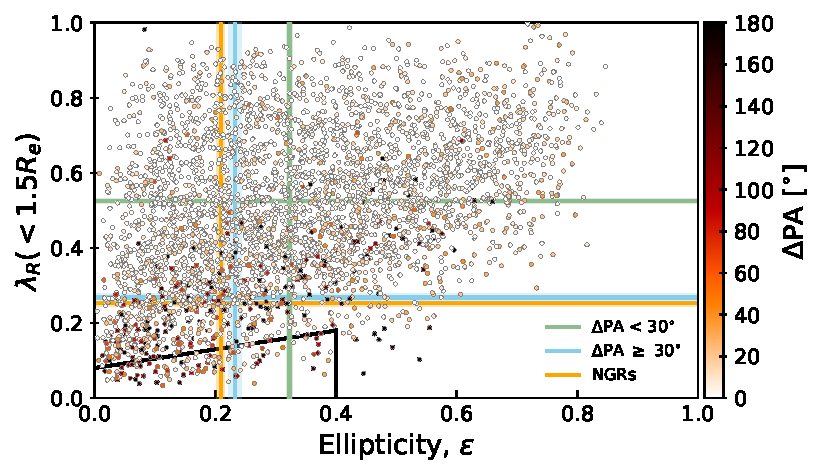
\includegraphics[width=\linewidth]{thesis/latex/misalignment_MaNGA/delPA_lambda_Re.pdf}
%     \caption{$\lambda_R$ within 1.5$\mathrm{R_e}$ against ellipticity, $\epsilon$ for all galaxies with defined $\Delta$PA. The individual points are for all $\Delta$PA defined MaNGA galaxies coloured by $\Delta$PA according to the colorbar. Medians for kinematically aligned ($\Delta$PA < 30$^{\circ}$), misaligned ($\Delta$PA > 30$^{\circ}$) and NGRs are shown by the green, light blue and orange lines respectively. The lighter shade around each line corresponds to the standard error. Aligned galaxies reside more typically in the fast rotator regime with higher $\lambda_R$ and $\epsilon$, whereas misaligned galaxies and NGRs reside closer to the slow rotator regime. The same qualitative trends are found if this plot is made for ETGs, S0-Sas or Sb-Sds alone.}
%     \label{fig:delPA_lambda_Re}
% \end{figure}

% In Figure \ref{fig:delPA_gasM} we show the distribution of gas masses for the aligned, misaligned and NGRs. We see a clear trend of lower gas mass going from kinematically aligned galaxies to misaligned galaxies to NGRs. We note that the majority ($\sim$80\%) of NGRs do not contain enough gas to have a measured gas mass from the routine of Pipe3D, so the distribution shown is a hard upper limit on the gas that these galaxies contain. We note that these trends remain qualitatively the same when considering the distributions for ETGs, S0-Sas and Sb-Sds individually.

% \begin{figure}
%     \centering
% 	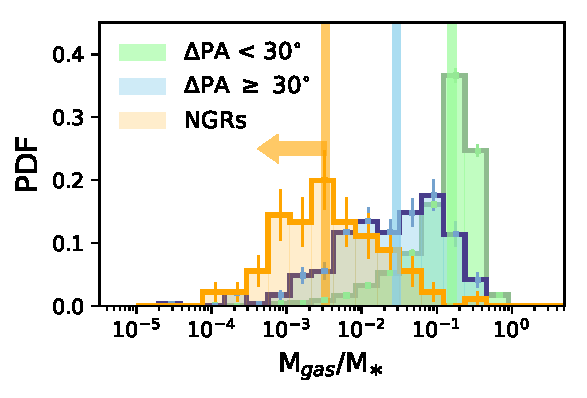
\includegraphics[width=0.8\linewidth]{misalignment_MaNGA/gas_mass_normed_all.pdf}
%     \caption{Probability density distributions of gas mass fraction, $\mathrm{(M_{gas}/M_{\ast})}$ for aligned galaxies ($\Delta$PA < 30$^{\circ}$) shown in green, those with high misalignment ($\Delta$PA > 30$^{\circ}$) in light blue and NGRs in orange. Each histogram is given with Poisson errors on each bin. The vertical lines denote the corresponding distribution's median. The majority of NGRs do not have detectable gas masses and therefore the distribution shown should be considered as upper bound.}
%     \label{fig:delPA_gasM}
% \end{figure}

% The similarity in stellar angular momentum between the NGRs and kinematically misaligned galaxies could indicate that they are from the same evolutionary sequence. A key component in decoupling star-gas rotation in simulations is a significant gas loss followed later by the accretion of material with misaligned angular momentum \citep[][]{vdvoort2015, starkenburg+19}. This gas loss can happen due to interactions from neighbouring galaxies which strips gas or through ejection due to black hole feedback.

% In \red{section halo assembly} \citet{duckworth2019a}, it was shown that kinematic decoupling shows little relationship with distance to filamentary structure. This could point to stripped/ejected material being re-accreted as a potential source of misalignment between star and gas rotation. Some NGRs could therefore represent an earlier timestamp before this material is re-accreted. Not all NGRs would necessarily re-accrete gas, meaning that some would remain quenched (and hence would not become misaligned in the future) potentially explaining the differences we see in stellar mass distributions of NGRs and misaligned. In this scenario, it would suggest that re-accretion of new material does not significantly alter the stellar angular momentum content going from NGRs to misaligned.

% \subsection{Morphology}
% We now sub-divide the total population by morphology into ETGs, S0-Sas and Sb-Sds as defined in \S\ref{sec:morph_def}. Figure \ref{fig:morph_PA}, shows the distributions for each category. We find that for all morphological types, galaxies are most commonly aligned with strong peaks below $\Delta$PA $\sim 30^{\circ}$. ETGs show a flatter distribution than their later counterparts, as the most likely to exhibit misalignment. LTGs show deeper drop-offs above $\Delta$PA $\sim 40^{\circ}$, with a boost around $\Delta$PA = 180$^{\circ}$, seen most strongly for the Sb-Sds. We quantify the overall misalignment fractions in the first column of Table \ref{tab:mega_table}. Our errors are estimated by binomial counting errors so that $\mathrm{\sigma = \sqrt{p(1-p) / M}}$ where $\mathrm{p = N/M}$ with $\mathrm{N}$ being the number of misaligned galaxies and $\mathrm{M}$ the total number of galaxies for the category.

% This morphological difference in misalignment is likely a result of several factors. Gas rich LTGs have typically higher specific angular momentum, and hence, require a higher magnitude gas inflow/outflow with different angular momentum to disrupt rotation and create misalignment. Conversely, ETGs are more dispersion dominated and gas poor enabling smaller gas in-flows (or outflows) to create a kinematic misalignment. 

% These results are reasonably consistent with previous findings of 36$\pm$5\% (of 260 galaxies) of ETGs that are misaligned in ATLAS\textsuperscript{3D} and in SAMI (45$\pm$6\% of 36 pure ellipticals, 5$\pm$1\% in 221 pure late spirals) \citep[][]{davis2011, bryant2019}. We note that our ETG misalignment fraction ($\sim$28\%) is lower than these previous findings and holds a slight tension with \citet{bryant2019}. Possible reasons for the differences may be due to morphology definition, stellar mass distribution or simply sample size. We note that enforcing stricter thresholds for morphology classifications doesn't change our misaligned fractions pointing to a likely difference in mass distributions or our increased sample size. 

% \begin{table*}
% \begin{tabular}{lllll}
% \hline
%         &  & All & Centrals & Satellites \\
% \hline
% All galaxies & $\Delta$PA defined &  3798 &  2185 &  1007 \\
% & $\Delta$PA $\geq 30^{\circ}$ &  420 (11.1$\pm$0.5\%) &  251 (11.5$\pm$0.7\%) &  102 (10.1$\pm$1.0\%) \\
% & NGR & 742 &  334 &  324 \\

% ETGs & $\Delta$PA defined & 301 & 204 & 97 \\
% & $\Delta$PA $\geq 30^{\circ}$ & 84 (27.9$\pm$2.6\%) & 60 (29.4$\pm$3.2\%) & 24 (24.7$\pm$4.4\%)  \\
% & NGR & 231 & 140 & 91 \\

% S0 - Sas & $\Delta$PA defined & 677 & 483 & 194 \\
% & $\Delta$PA $\geq 30^{\circ}$ &  66 (9.7$\pm$1.1\%) & 49 (10.1$\pm$1.4\%) & 17 (8.8$\pm$2.0\%) \\
% & NGR & 100 & 44 & 56 \\

% Sb - Sds & $\Delta$PA defined & 1634 & 1112 & 522 \\
% & $\Delta$PA $\geq 30^{\circ}$ & 88 (5.4$\pm$0.6\%) & 58 (5.2$\pm$0.7\%) & 30 (5.7$\pm$1.0\%) \\
% & NGR & 107 & 32 & 75 \\

% \end{tabular}
% \caption{Total number of galaxies used in this study for each of $\Delta$PA defined sample, of those that are kinematically misaligned and those that have well defined stellar rotation but incoherent gas (NGR). These are defined for both splitting on morphology (rows) and group membership (columns). For those that are kinematically misaligned ($\Delta$PA $\geq 30^{\circ}$), the percentage with respect to all those with $\Delta$PA measurements for the sub-category is shown. The uncertainties quoted are binomial counting errors.}
% \label{tab:mega_table}
% \end{table*}

% The boost in the PDF around 180$^{\circ}$ of Figure \ref{fig:morph_PA} suggests that near counter-rotation is a stable state for galaxies. This is seen most prominently in Sb-Sds with a clear upwards trend in the PDF from $\sim$140$^{\circ}$. A possible explanation is that these rotation dominated galaxies host strong stellar torques, which act to realign gas at intermediate misalignments ($30^{\circ} < \Delta$PA $ < 150^{\circ}$) on much faster timescales than in ETGs. Counter-rotators, however, remain stable and hence contribute proportionally higher to the misaligned distribution, in comparison to those at intermediate misalignments which settle towards alignment or counter-rotation.

% Interestingly galaxies that exhibit near-counter rotation ($\Delta$PA $\geq$ 150$^{\circ}$) have similar stellar angular momentum to the general misaligned population ($\Delta$PA $\geq$ 30$^{\circ}$), significantly lower than the aligned counterparts. This holds true for all morphologies. \citet{chen2016} previously highlighted the boost in star formation in central regions for counter-rotating LTGs. As suggested, this could be a natural result of cancellation of angular momentum leading to increased in-flows to central regions. Our finding of lowered angular momentum in the counter-rotators (with respect to the co-rotators) supports this claim.

% \begin{figure}
% 	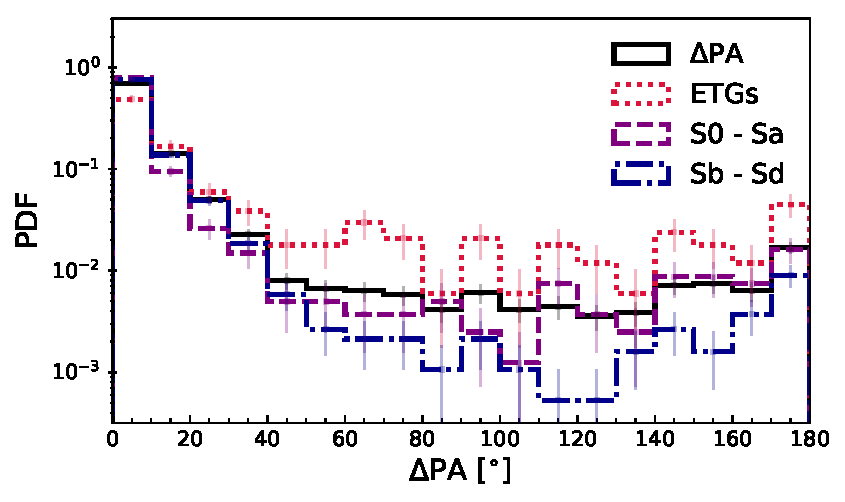
\includegraphics[width=\linewidth]{thesis/latex/misalignment_MaNGA/delPA_morph.pdf}
%     \caption{Probability density distributions of kinematic misalignment as defined by $\Delta$PA split on morphology. The probability density distribution is normalised to 1 and shown in log scale. Distributions for the total population, ETGs, S0/Sa and Sb-Sds are shown by black solid, dotted red, dashed purple and dot-dashed blue lines respectively. Earlier type galaxies are more likely to be misaligned than later type galaxies.}
%     \label{fig:morph_PA}
% \end{figure}

% Due to the relationship between stellar mass, morphology and specific angular momentum \citep[e.g.][]{cortese2016}, it might be expected that misaligned galaxies should be at higher stellar mass due to their lower $\mathrm{\lambda_{R}}$ with respect to the aligned \citep[see also;][]{bryant2019}. Surprisingly for the overall population we see little difference, however, splitting on morphology as shown in Figure \ref{fig:morph_stelM} reveals individual trends. Misaligned ETGs (and NGRs) are more massive than the aligned counterparts most likely indicative that misaligned galaxies have had richer merger histories. The opposite trends are seen for both S0-Sas and Sb-Sds with kinematically aligned galaxies being of typically higher mass than the misaligned. This could be indicative that the pathways leading to misalignment are different as a function of morphology.

% \begin{figure}
%     \centering
% 	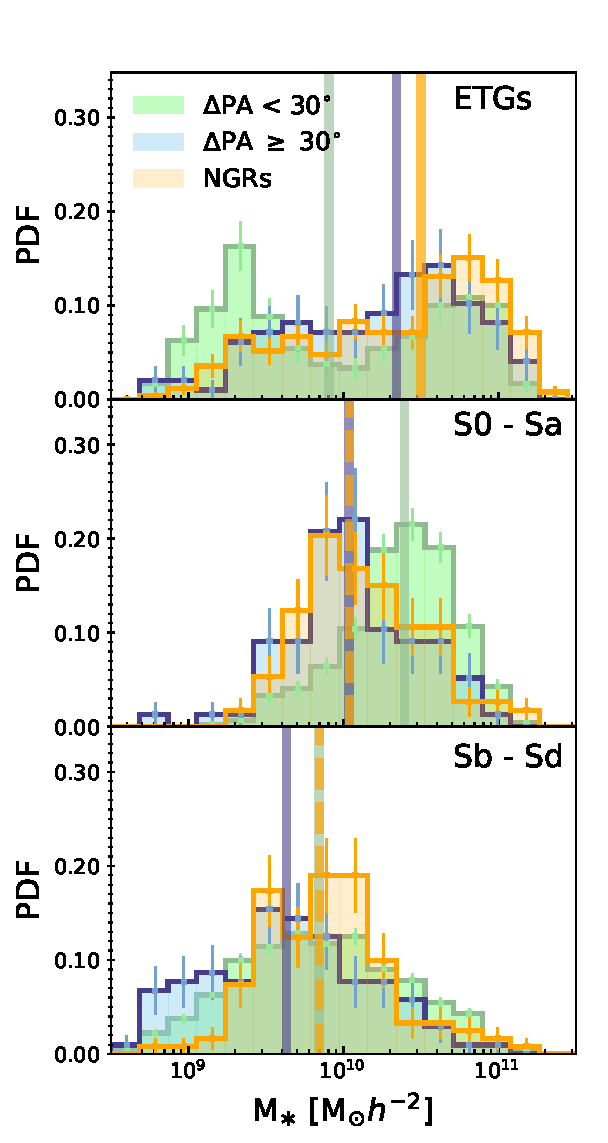
\includegraphics[width=0.5\linewidth]{thesis/latex/misalignment_MaNGA/delPA_stelM_morph_nsa.pdf}
%     \caption{Probability density distributions of stellar mass, $\mathrm{(M_{\ast}/M_{\odot})}$ for aligned galaxies ($\Delta$PA < 30$^{\circ}$, misaligned galaxies ($\Delta$PA > 30$^{\circ}$) and NGRs for ETGs, S0-Sas and Sb-Sds (top to bottom). In each panel the aligned/misaligned are shown with solid lines with the aligned in the darker shade. NGRS are shown by dot-dashed lines. Each histogram is given with Poisson errors on each bin. The vertical lines denote the corresponding distribution's median. For ETGs, aligned galaxies are less massive than the misaligned sample. This trend, however, reverses for S0-Sas and Sb-Sds.}
%     \label{fig:morph_stelM}
% \end{figure}

% \subsection{Group membership}
% Group membership is important for dictating the evolution of a galaxy and hence we now sub-divide our population into centrals and satellites as described in \S\ref{sec:group_def}. Figure \ref{fig:group_morph_PA} (top panels) shows the $\Delta$PA distributions as in Figure \ref{fig:morph_PA}, but now split into centrals and satellites. Qualitatively the morphological trends remain however Table \ref{tab:mega_table} reveals that centrals (29.4$\pm$3.2\%) are slightly more likely to be misaligned than satellites (24.7$\pm$4.4\%) for ETGs. This is also potentially seen for the S0-Sbs (10.1$\pm$1.4\% for centrals vs 8.8$\pm$2.0\% for satellites), however we note that both fractions are within each other's errorbars.

% \begin{figure*}
%     \centering
% 	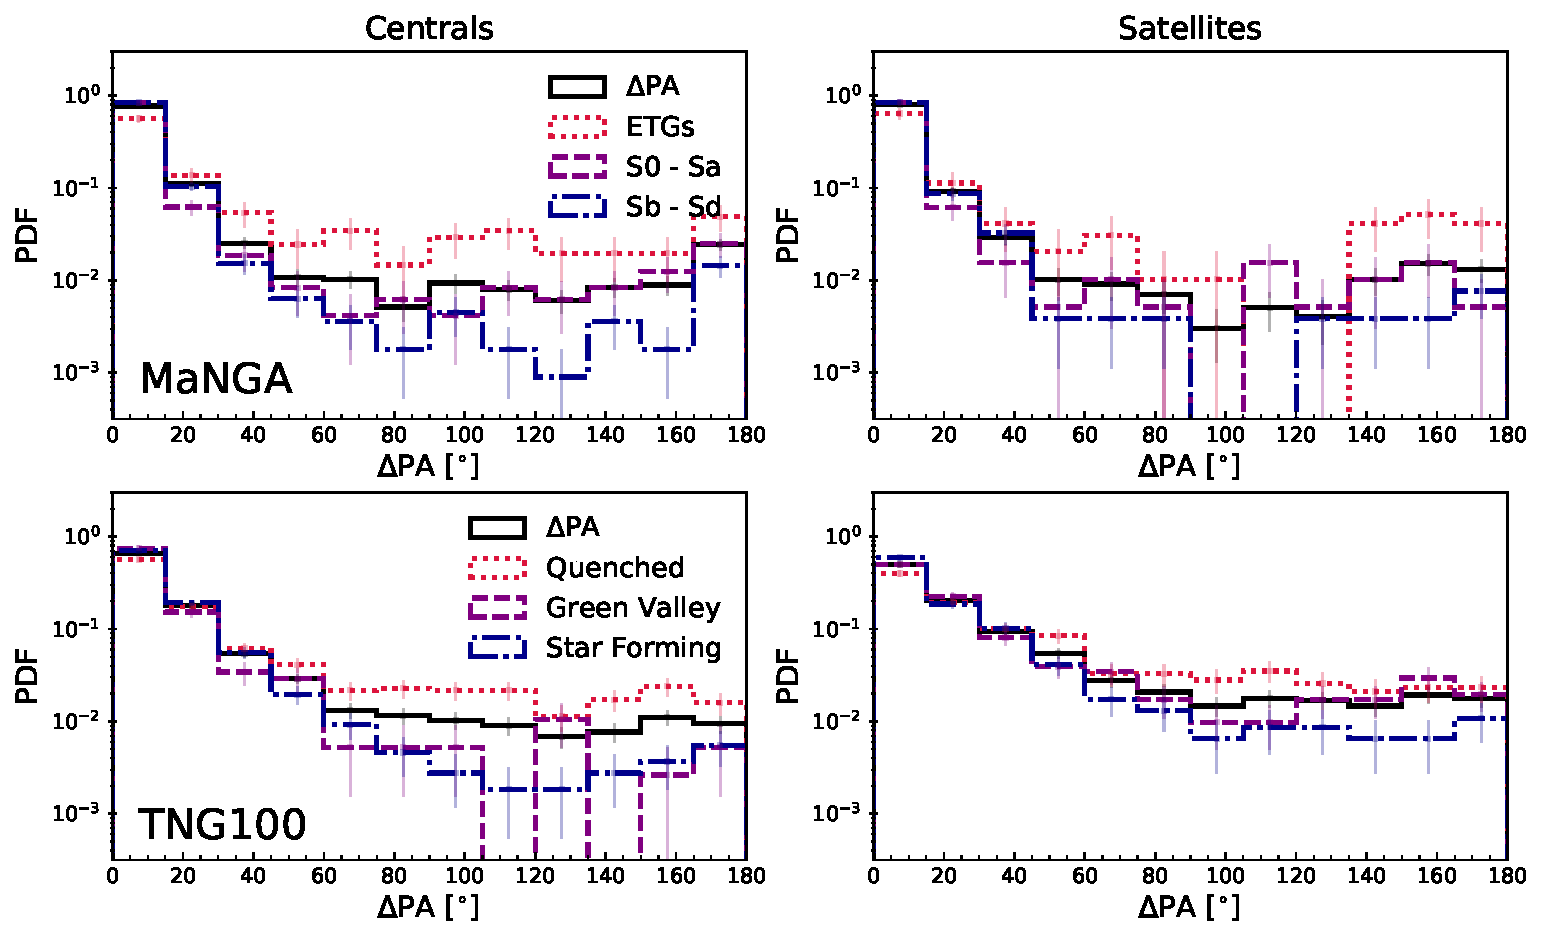
\includegraphics[width=\linewidth]{misalignment_MaNGA/MPL8_TNG_morph_group_PA.pdf}
%     \caption{Same as Figure \ref{fig:morph_PA}, however split by group membership into centrals (left) and satellites (right). The top panel shows for the MaNGA sample and the bottom shows for the mock sample in TNG100. Morphology for TNG100 is categorised by the deviation of the galaxy's star formation away from the main sequence of galaxies in the whole of TNG100 (see \S\ref{sec:tng_results})}
%     \label{fig:group_morph_PA}
% \end{figure*}

% Figure \ref{fig:group_morph_stelM} shows the stellar mass distribution for our samples but now additionally split into centrals and satellites. Again we find the same qualitative trends for both centrals and satellites; i.e. misaligned ETGs are more massive than their aligned counterparts whereas misaligned S0-Sas and Sb-Sds are less massive than those aligned.
% \begin{figure*}
%     \centering
% 	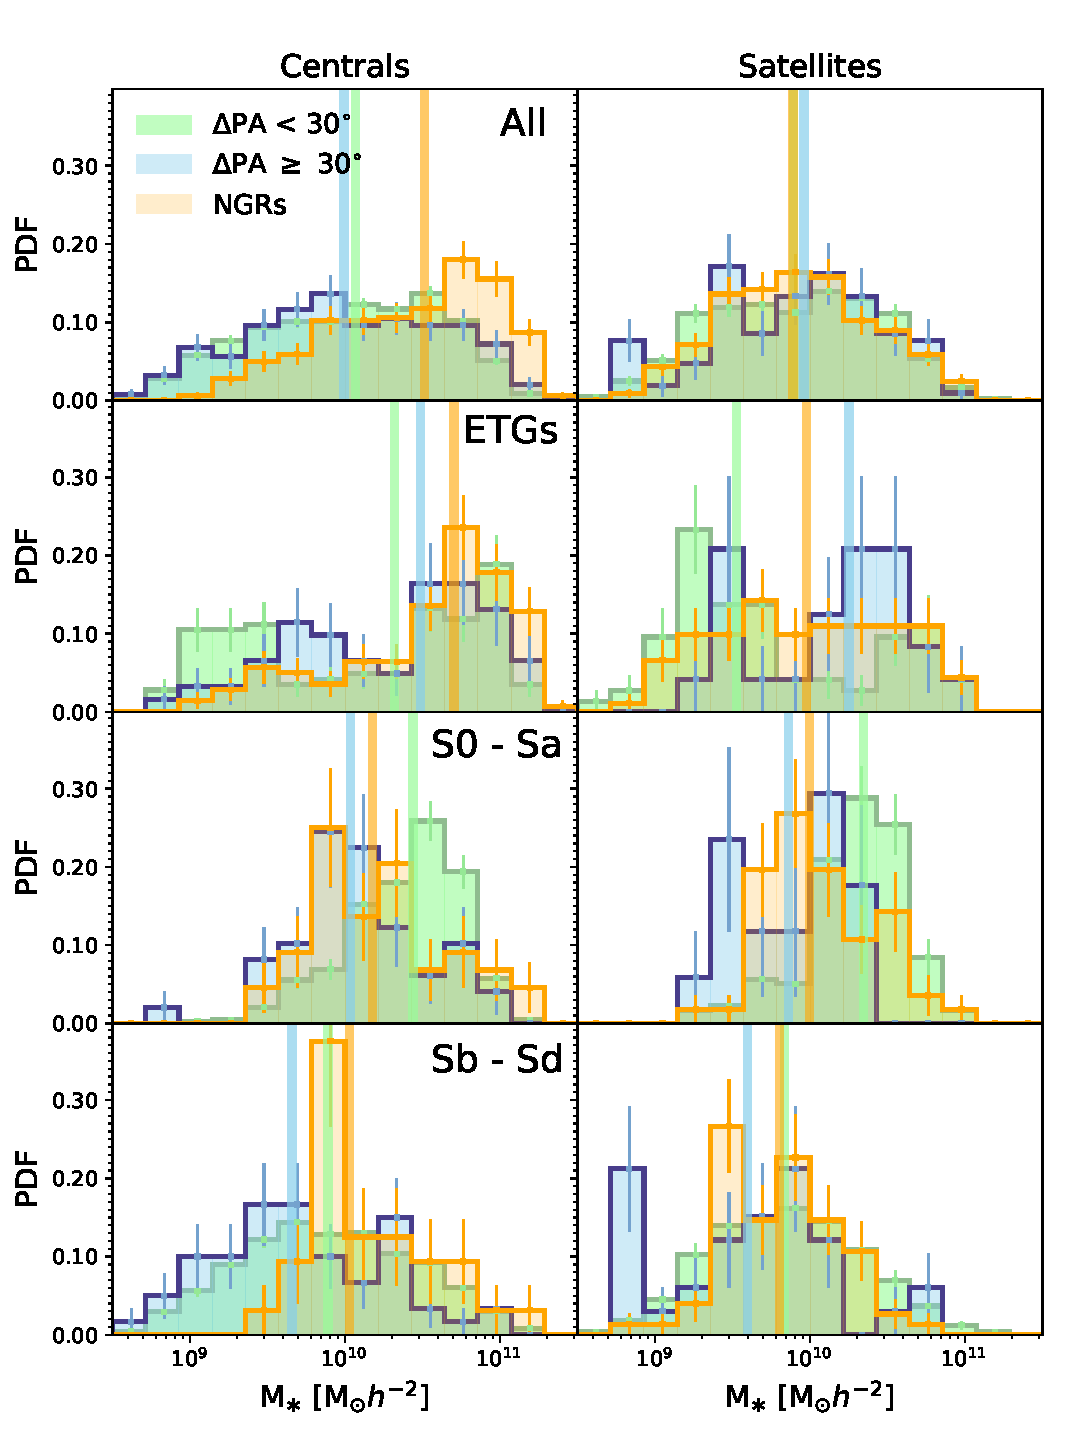
\includegraphics[width=0.85\linewidth]{misalignment_MaNGA/delPA_stelM_morph_lim_nsa.pdf}
%     \caption{Same as Figure \ref{fig:morph_stelM}, however split by group membership into centrals (left) and satellites (right). Additionally the distributions for the overall central and satellite populations is shown in the top row. We see that for ETGs there is a strong difference in mass between aligned and misaligned satellites. This trend is reversed for S0/Sa and Sb/Sd satellites. These trends are also seen for centrals, however, typically to a lesser degree.}
%     \label{fig:group_morph_stelM}
% \end{figure*}

% \section{Summary}
% In this chapter, we introduce a catalogue of $\sim$4500 galaxies from the MaNGA survey in order to establish the
% prevalence of misalignment as a function of optical morphology. We also relate the typical stellar angular momentum and gas content of kinematically misaligned galaxies relative to the aligned. Our conclusions are as follows:

% \begin{enumerate}
%     \item The prevalence of kinematic misalignment (i.e. where rotational axes of stars and gas are offset by $> 30^{\circ}$) is strongly morphological dependent with ETGs having $\sim$28\% exhibiting misalignment which decreases to $\sim$5\% for Sb-Sds.
    
%     \item For all morphologies this misalignment is related to a lowered stellar angular momentum and also a lowered gas mass. We note that misaligned galaxies have similar stellar angular momentum to those do not have coherently rotating gas (those with large gas depletion fall into this category). This could be indicative that galaxies without coherent gas rotation and kinematically misaligned galaxies are different timesteps in the same evolutionary sequence. As noted in simulations \citep[][]{vdvoort2015, starkenburg+19}, a key component in decoupling star-gas rotation is a significant gas loss followed by accretion of new gas with misaligned angular momentum. In this scenario, NGRs could represent an earlier timestamp before a future re-accretion of gas. This would indicate that the stellar angular momentum is disrupted prior to accretion of new material. 
    
%     \item We find that the misalignment fraction is also dependent on group membership. For ETGs and S0-Sas, central galaxies are more likely to exhibit misalignment than satellites. For Sb-Sds this trend reverses.
    
%     \item We find that counter-rotation (i.e. rotational axes of stars and gas are offset by $> 150^{\circ}$) is a stable state for galaxies of all morphologies shown by a boost in the PDF (Figure \ref{fig:morph_PA}). Similar to the total misaligned population, counter-rotators have distinctly lower angular momentum than their aligned counterparts. 

% \end{enumerate}

% In the following chapter, we investigate whether hydrodynamical simulations can reproduce these observed trends and what typical timescales are associated with angular momentum and gas loss.